\documentclass[conference]{IEEEtran}
\IEEEoverridecommandlockouts

\usepackage[english]{babel}
\usepackage{amsmath,amssymb}
\usepackage{graphicx}
\usepackage{textcomp}
\usepackage{booktabs}
\usepackage{url}
\usepackage[hidelinks]{hyperref}
\usepackage{cite}
\usepackage{array}
\usepackage{microtype}
\usepackage{multirow}

% Place image files in the same Overleaf project folder as this .tex, or in a subfolder 'figures/'.
\graphicspath{{./}{./figures/}}

\title{GraphRAG Social Intelligence: End-to-End GNN, Retrieval, API, and Web Frontend for Social Network Analysis}

\author{%
\IEEEauthorblockN{Neeraj Yadav\textsuperscript{*},
Dev Singh\textsuperscript{**},
Gourav Varanasi}%
\IEEEauthorblockA{\textit{Department of Computer Science}\\
\textit{Shiv Nadar University}\\
Greater Noida, India\\
\textsuperscript{*}Student ID: 2310110199 \quad
\textsuperscript{**}Student ID: 2310110099}%
}

\begin{document}
\maketitle

\begin{abstract}
We present a complete social network intelligence system that combines (i) exploratory and production training notebooks for retrieval-only (RAG), graph-only (GNN), and GNN\,$+$\,semantic hybrid models on the SNAP Facebook page--page network and Twitter ego data; (ii) a Neo4j backend with property-graph schema and native vector indexes for hybrid Cypher\,$+$\,vector retrieval; (iii) a FastAPI service exposing health, graph analytics, multi-agent GraphRAG chat, and optional natural-language inserts; (iv) GPU training on Kaggle and CPU-oriented inference; (v) Docker Compose orchestration for Neo4j and the API; and (vi) a Next.js frontend for dashboards, chat, and graph exploration. This final report unifies the mid-term methodology with repository-scale implementation, API documentation, deployment, and \textbf{exact} evaluation numbers recovered from the executed notebook outputs (Kaggle, 2026 runs).
\end{abstract}

\begin{IEEEkeywords}
Graph neural networks, GraphRAG, Neo4j, vector search, FastAPI, Kaggle, Docker, social networks, knowledge-augmented generation, node classification.
\end{IEEEkeywords}

\section{Introduction}

Social graphs encode \emph{who links to whom} and metadata about users and content. Text-only retrieval underuses topology; graph-only models may ignore semantics in text. This project fuses \textbf{Graph Neural Networks} (GNNs) for structure-aware prediction, \textbf{hybrid retrieval} (graph Cypher and vector similarity) in Neo4j, and a \textbf{multi-agent} pipeline (analysis, routing, retrieval, GNN scoring, LLM synthesis, validation) to support both API consumers and an interactive web UI \cite{project_readme,project_explain,feature_readme}.

\section{Related Work and Positioning}

We align with the literature on combining graph machine learning and large language models: graphs provide relational bias and grounding; LLMs offer flexible natural-language interfaces \cite{acm_survey_gml_llm}. Encoder choices follow GraphSAGE \cite{hamilton2017graphsage} and PyG tooling \cite{pyg}, with graph and vector co-location in Neo4j \cite{neo4j_vector,arch_md}. The present work extends a mid-term report \cite{midterm_internal} to the full system in the repository: notebooks, Kaggle training, API, Docker, and frontend \cite{frontend_api_guide}.

\section{Datasets and Notebook Experiments}

Training and exploration use (a) the SNAP \textbf{Facebook} page--page network (MUSAE-style CSVs; four page-type classes) and (b) \textbf{Twitter} ego networks via PyG \texttt{SNAPDataset} (four activity-tier classes). RAG-only notebooks embed per-node text descriptions with \texttt{sentence-transformers/all-MiniLM-L6-v2} and query an LLM with retrieved context; GNN and GNN\,$+$\,RAG notebooks report test metrics after training. Table~\ref{tab:nbmetrics} gives \textbf{verbatim} numbers from the bottom of the saved notebook outputs (executed Kaggle environment; Git-tracked \texttt{.ipynb} in \texttt{notebooks/}).

\begin{table*}[t]
\centering
\caption{Exact summary lines from notebook outputs (see filenames). RAG-only rows report embedding preparation; GNN and GNN\,$+$\,RAG rows report test metrics.}
\label{tab:nbmetrics}
\small
\begin{tabular}{@{}l p{0.45\linewidth}@{}}
\toprule
\textbf{Notebook} & \textbf{Key output (verbatim from run)} \\
\midrule
\texttt{rag-only-pipeline-facebook.ipynb} & \texttt{Total nodes: 22470};\quad \texttt{Embedding shape: (22470, 384)} \\
\texttt{rag-only-pipeline-twitter.ipynb} & \texttt{Total nodes: 133857};\quad \texttt{Embedding shape: (133857, 384)} \\
\texttt{gnn-only-facebook.ipynb} & \texttt{Test size: 4494};\quad \texttt{Total nodes used: 22470};\quad \texttt{Test Accuracy: 0.9306 | F1 (macro): 0.9278 | AUC (macro OVR): 0.9880} \\
\texttt{gnn-only-twitter.ipynb} & \texttt{Nodes: 133857 X: (133857, 385) edges listed: 3549272};\quad \texttt{Feature shape: (133857, 385)}; last line: \texttt{Loaded best val checkpoint: val acc 0.8794, test acc at save 0.8727 -> weights/best.pth} (final epoch line: \texttt{Epoch~26} \texttt{Test Acc: 0.8628 | Test F1: 0.8540 | Test AUC: 0.9846}) \\
\texttt{gnn-rag-facebook-best.ipynb} & \texttt{Test Accuracy: 0.9437 | F1 (macro): 0.9412 | AUC (macro OVR): 0.9918};\quad \texttt{Train Acc: 0.9559 | F1: 0.9532 | AUC: 0.9943};\quad \texttt{Test Acc: 0.9437 | F1: 0.9412 | AUC: 0.9918} \\
\texttt{gnn-rag-twitter-best.ipynb} & \texttt{Data(x=[133857, 769], edge\_index=[2, 3549272], y=[133857]) | graph\_feat\_dim: 385 | text dim: 384};\quad \texttt{Test Accuracy: 0.9746 | F1 (macro): 0.9704 | AUC (macro OVR): 0.9920};\quad \texttt{Early stop: \ldots\ Best val acc=0.9727, test acc at that checkpoint} $\sim$ \texttt{0.9742};\quad final summary: \texttt{Train Acc: 0.9744 | F1: 0.9699 | AUC: 0.9931} and \texttt{Test Acc: 0.9748 | F1: 0.9707 | AUC: 0.9920} \\
\bottomrule
\end{tabular}
\end{table*}

\noindent\textbf{Interpretation.} RAG-only pipelines do not emit a single accuracy; they report scale and dense embedding shape. For Facebook, GNN-only test accuracy is 0.9306; the GNN\,$+$\,semantic hybrid (\texttt{gnn-rag-facebook-best.ipynb}) reaches \textbf{0.9437} test accuracy. For Twitter, the GAT-style training in \texttt{gnn-only-twitter.ipynb} selects a best checkpoint with test accuracy \textbf{0.8727} at save; the GNN\,$+$\,text hybrid in \texttt{gnn-rag-twitter-best.ipynb} achieves a higher reported test accuracy (\textbf{0.9746} in the test-evaluation line; summary lines show \textbf{0.9748} test acc). The Twitter hybrid notebook shows oscillating per-epoch test metrics, consistent with aggressive learning-rate or sampling schedules; the early-stopping and final evaluation lines in the same notebook should be cited together.

\begin{figure*}[t]
\centering
\begin{tabular}{@{}ccc@{}}
\includegraphics[width=0.31\linewidth]{fig_rag_facebook} &
\includegraphics[width=0.31\linewidth]{fig_rag_twitter} &
\includegraphics[width=0.31\linewidth]{fig_gnn_facebook} \\
\small (a) RAG Facebook & \small (b) RAG Twitter & \small (c) GNN Facebook
\end{tabular}\\[0.5em]
\begin{tabular}{@{}ccc@{}}
\includegraphics[width=0.31\linewidth]{fig_gnn_twitter} &
\includegraphics[width=0.31\linewidth]{fig_gnn_rag_facebook} &
\includegraphics[width=0.31\linewidth]{fig_gnn_rag_twitter} \\
\small (d) GNN Twitter & \small (e) GNN\,$+$\,RAG Facebook & \small (f) GNN\,$+$\,RAG Twitter
\end{tabular}
\caption{Notebook evidence: use screenshots of final cells (metrics or embedding lines) for (a)--(f). See \texttt{docs/Presentation\_readme.md} for how to export from Kaggle or locally.}
\label{fig:notebooks}
\end{figure*}

\section{System Architecture}

\subsection{Runtime pipeline}
The API orchestrates: Query Analyzer $\rightarrow$ Router $\rightarrow$ Retrievers (graph Cypher, vector ANN, optional fusion) $\rightarrow$ GNN inference (CPU) $\rightarrow$ Synthesizer (KAG) $\rightarrow$ Validator \cite{project_readme,feature_readme}. Figure~\ref{fig:arch} matches the repository README flow.

\begin{figure}[t]
\centering
\includegraphics[width=0.95\linewidth]{architecture_diagram}
\caption{Multi-agent query pipeline (conceptual; reuse project diagram asset).}
\label{fig:arch}
\end{figure}

\subsection{Neo4j as unified graph and vector store}
The implementation consolidates on Neo4j: text embeddings and GNN embeddings on nodes, multiple vector indexes by dimension, hybrid Cypher for hot paths, and Python-side reciprocal-rank fusion when two query shapes must merge \cite{arch_md}. Figure~\ref{fig:neo4j} illustrates a Browser or equivalent view of the property graph and indexes.

\begin{figure}[t]
\centering
\includegraphics[width=0.95\linewidth]{neo4j}
\caption{Neo4j: schema and/or vector index context (screenshot from Neo4j Browser).}
\label{fig:neo4j}
\end{figure}

\subsection{Model code and inference}
The \texttt{model/} package implements \texttt{SocialGraphGNN} and related heads; \texttt{model/inference.py} provides CPU-only inference. Training scripts under \texttt{training/} mirror dataset-specific Kaggle entry points described in the README (Facebook, Twitter, Reddit).

\section{Backend service layer}
The FastAPI entry point is \texttt{api/main.py}. The process groups concerns as follows: \textbf{operations} (connectivity, dataset counts, GNN and vector state); \textbf{ingestion} (bulk load and status of prepared datasets); \textbf{conversational GraphRAG} (multi-agent pipeline for natural language and a lighter program-facing path to the same engine); \textbf{direct graph analytics} (read-only, parameterized Cypher in \texttt{GraphQueryService} for tables and charts with minimal latency); and \textbf{optional inserts} (natural-language and structured graph writes, feature-gated by configuration). Response envelopes include \texttt{insight}, \texttt{validation}, and \texttt{pipeline\_timing\_ms} for transparency. Integration wire details are in the repository guide \cite{frontend_api_guide}. Figure~\ref{fig:swagger} shows the auto-generated OpenAPI browser shipped with the framework.

\begin{figure}[t]
\centering
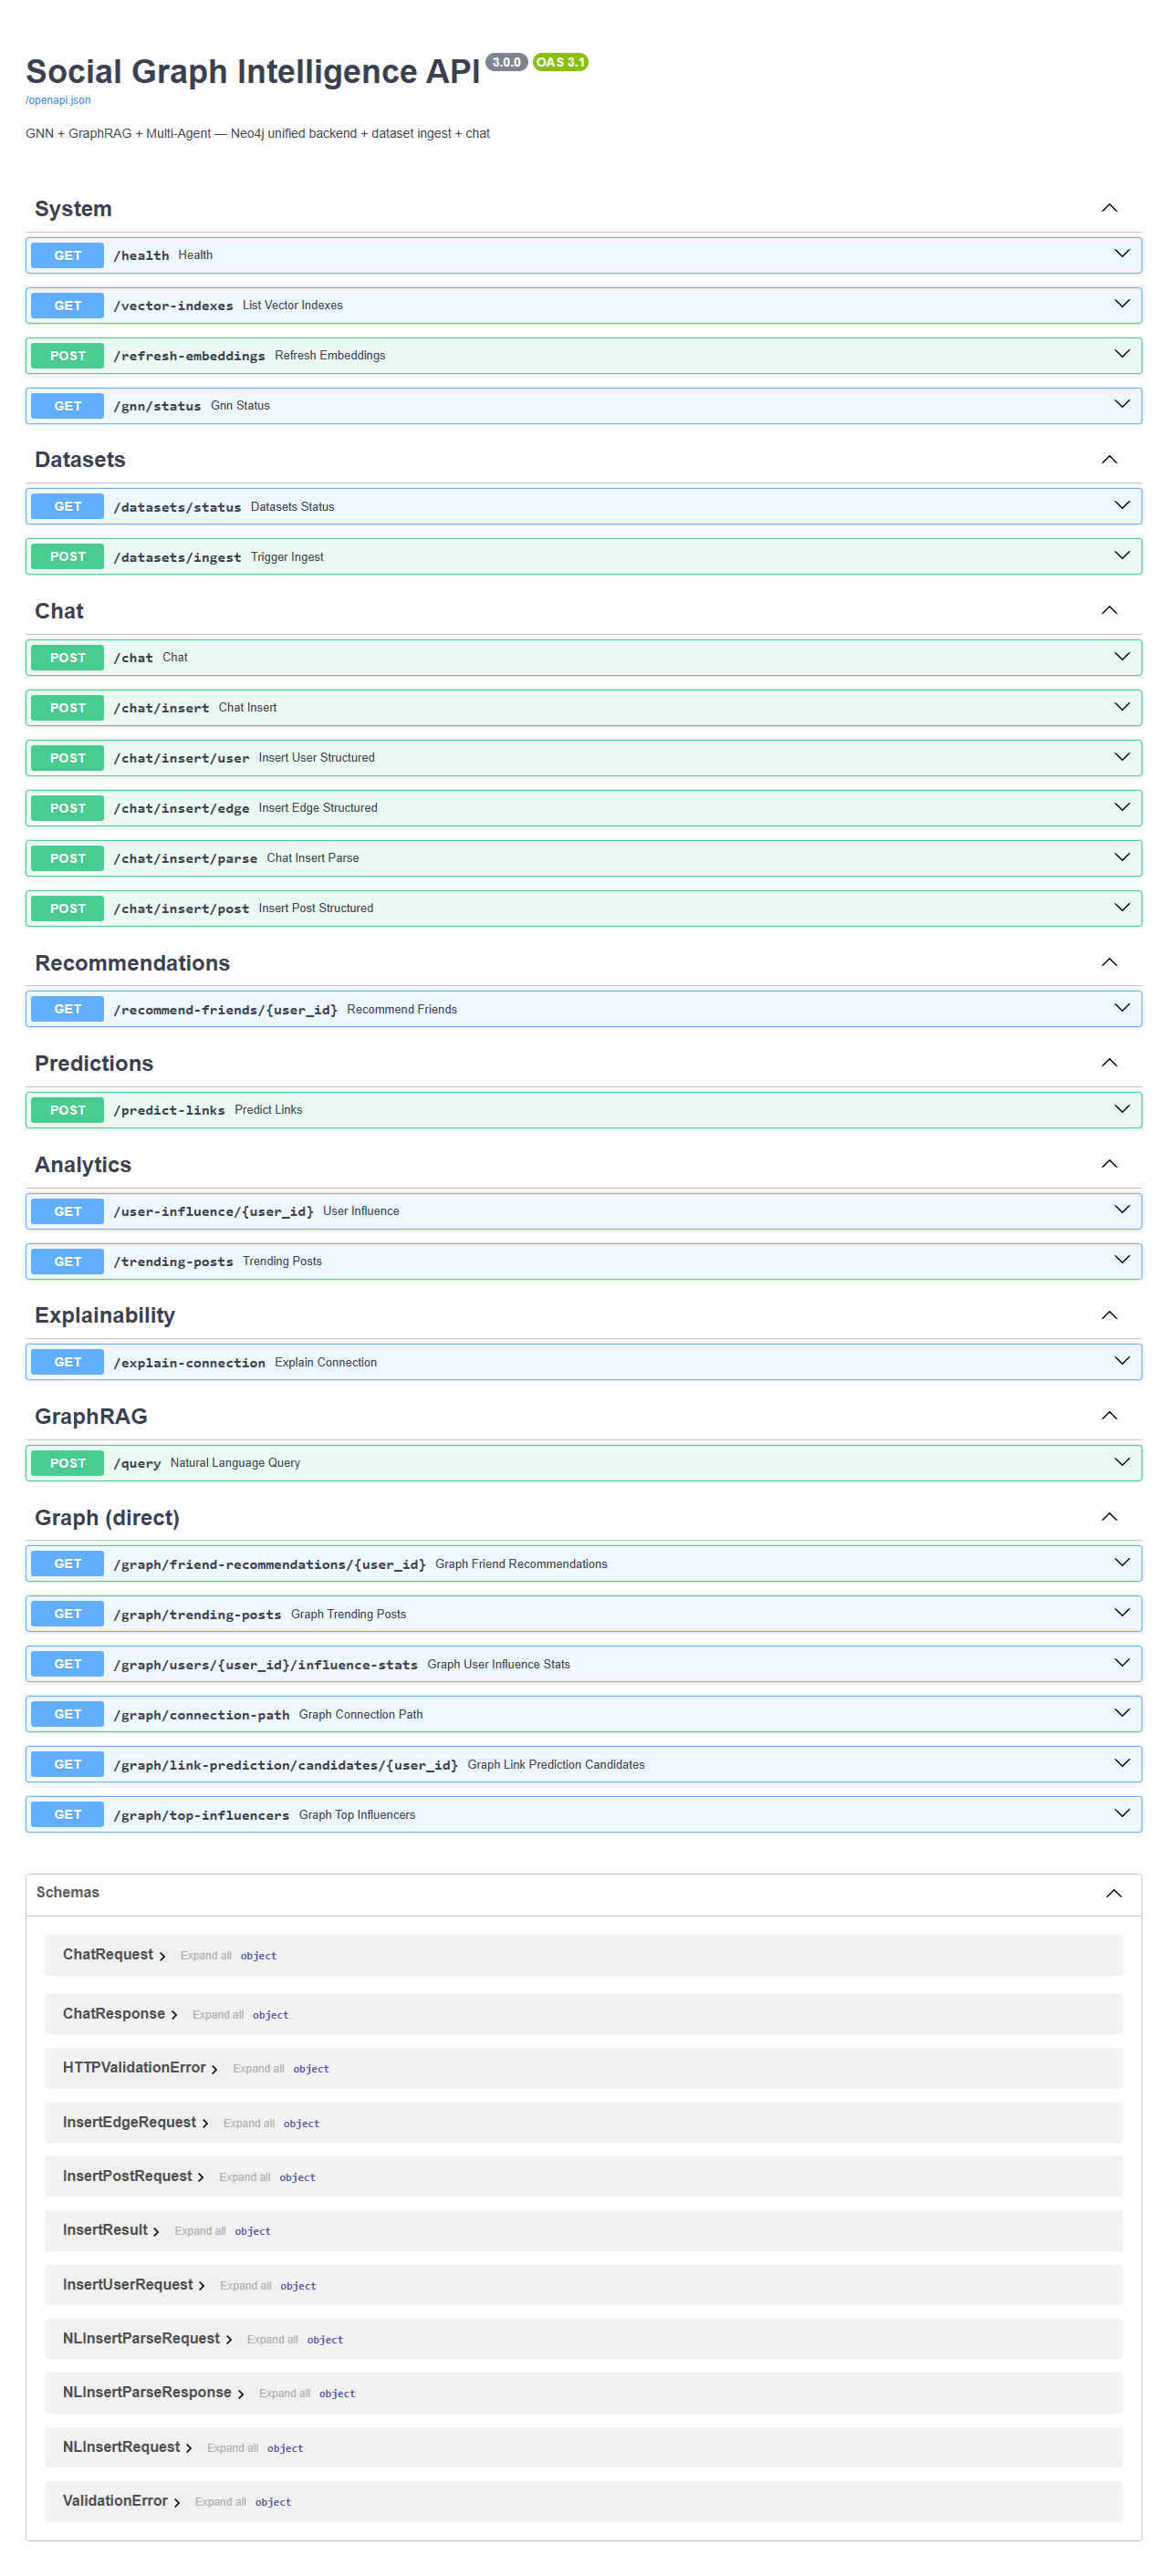
\includegraphics[width=0.95\linewidth]{fig_swagger}
\caption{FastAPI interactive API schema and try-it-out view after \texttt{uvicorn} or Docker—capture from the live server.}
\label{fig:swagger}
\end{figure}

\section{Kaggle Training Workflow}
Kaggle GPU notebooks (2026) host \texttt{notebooks/*.ipynb} and \texttt{training/*.py}. Procedure: attach the Facebook dataset where required; set output to \texttt{/kaggle/working}; download \texttt{model\_weights\_*.pth} and \texttt{embeddings\_*.npy} into the repository \texttt{weights/} directory for local or Docker inference \cite{project_readme}.

\section{Docker Deployment}
\texttt{docker/docker-compose.yml} runs Neo4j 5.13 (ports 7474, 7687) and the API (port 8000) on a shared network; the API image mounts \texttt{weights/} read-only and expects \texttt{NEO4J\_URI=bolt://neo4j:7687}. Health checks use \texttt{cypher-shell} for the database and an HTTP probe against the API process \cite{docker_compose_repo}. Figure~\ref{fig:docker} can show \texttt{docker compose ps} or the Docker Desktop view.

\begin{figure}[t]
\centering
\includegraphics[width=0.95\linewidth]{fig_docker}
\caption{Docker: compose services healthy (terminal or Docker UI screenshot).}
\label{fig:docker}
\end{figure}

\section{Frontend}
A Next.js application (not fully reproduced in this \texttt{docs/} tree) provides screens for the dashboard, AI chat, graph exploration, analytics, user profiles, path finding, and admin ingestion—each backed by the service capabilities described in the feature documentation \cite{feature_readme,frontend_api_guide}. Figure~\ref{fig:ui} is a recommended dashboard or chat capture.

\begin{figure}[t]
\centering
\includegraphics[width=0.95\linewidth]{fig_frontend_dashboard}
\caption{Frontend: e.g., dashboard with health cards and dataset stats, or the chat view with per-stage timings.}
\label{fig:ui}
\end{figure}

\section{Testing}
The \texttt{tests/} tree includes service and model tests. Running \texttt{pytest tests/} validates critical paths. Optional pipeline accuracy checks (e.g., stratified splits) align with the mid-term testing narrative \cite{midterm_internal}.

\section{Conclusion}
We described an integrated stack: verified notebook metrics on Facebook and Twitter, Neo4j-centric GraphRAG, a production-style FastAPI split between a conversational pipeline and a direct graph query service, Kaggle training outputs for weights, containerized deployment, and a feature-complete frontend. Future work: tighter latency budgets for vector search at scale, extended Reddit evaluation, and production hardening (CORS, auth, and insert policies).

\section*{Acknowledgment}
The authors thank Shiv Nadar University and the Department of Computer Science for support of this project.

\bibliographystyle{IEEEtran}
\begin{thebibliography}{00}

\bibitem{acm_survey_gml_llm}
``Graph Machine Learning in the Era of Large Language Models,'' \emph{ACM Comput. Surv.}, 2025.

\bibitem{project_readme}
``Social Network Intelligence System'' (README), GraphRAG Social Intelligence repository, 2025--2026.

\bibitem{project_explain}
``GraphRAG Social Intelligence System: Complete Project Explanation,'' \texttt{project\_explanation\_readme.md}, repository, 2025--2026.

\bibitem{feature_readme}
``Feature \& Architecture Explanation'' (frontend screens), \texttt{feature\_explanation\_readme.md}, repository, 2025--2026.

\bibitem{frontend_api_guide}
``Frontend integration guide—Social Graph Intelligence API,'' \texttt{docs/FRONTEND\_API\_GUIDE.md}, repository, 2025--2026.

\bibitem{arch_md}
``Neo4j-Only Architecture: Design Decisions \& Performance Analysis,'' \texttt{ARCHITECTURE.md}, repository, 2025--2026.

\bibitem{midterm_internal}
N.~Yadav, D.~Singh, and G.~Varanasi, ``Enhancing Graph Neural Networks with Retrieval-Augmented Generation for Node Classification,'' mid-term report, \texttt{docs/IEEE\_Midterm\_Report\_Overleaf.tex}, 2026.

\bibitem{hamilton2017graphsage}
W.~L. Hamilton, R.~Ying, and J.~Leskovec, ``Inductive representation learning on large graphs,'' in \emph{Proc. NeurIPS}, 2017.

\bibitem{pyg}
M.~Fey and J.~E. Lenssen, ``Fast graph representation learning with PyTorch Geometric,'' in \emph{ICLR Workshop on Representation Learning on Graphs and Manifolds}, 2019.

\bibitem{neo4j_vector}
Neo4j, ``Vector indexes,'' \url{https://neo4j.com/docs/cypher-manual/current/indexes-for-vector-search/}

\bibitem{docker_compose_repo}
``social\_graph\_intelligence'' \texttt{docker/docker-compose.yml}, GraphRAG Social Intelligence repository, 2025--2026.

\end{thebibliography}

\end{document}
